\documentclass{exam}
%\documentclass[11pt,a4paper]{exam}
\usepackage{amsmath,amsthm,amsfonts,amssymb,dsfont}
\usepackage{ifthen}
\usepackage{enumerate}% http://ctan.org/pkg/enumerate
\usepackage{multicol}
\usepackage{hyperref}
\usepackage{graphicx}
\usepackage{float}

% Accumulate the answers. Unmodified from Phil Hirschorn's answer
% https://tex.stackexchange.com/questions/15350/showing-solutions-of-the-questions-separately/15353
\newbox\allanswers
\setbox\allanswers=\vbox{}

\newenvironment{answer}
{%
    \global\setbox\allanswers=\vbox\bgroup
    \unvbox\allanswers
}%
{%
    \bigbreak
    \egroup
}

\newcommand{\showallanswers}{\par\unvbox\allanswers}
% End Phil's answer


% Is there a better way?
\newcommand*{\getanswer}[5]{%
    \ifthenelse{\equal{#5}{a}}
    {\begin{answer}\thequestion. (a)~#1\end{answer}}
    {\ifthenelse{\equal{#5}{b}}
        {\begin{answer}\thequestion. (b)~#2\end{answer}}
        {\ifthenelse{\equal{#5}{c}}
            {\begin{answer}\thequestion. (c)~#3\end{answer}}
            {\ifthenelse{\equal{#5}{d}}
                {\begin{answer}\thequestion. (d)~#4\end{answer}}
                {\begin{answer}\textbf{\thequestion. (#5)~Invalid answer choice.}\end{answer}}}}}
}

\setlength\parindent{0pt}
%usage \choice{ }{ }{ }{ }
%(A)(B)(C)(D)
\newcommand{\fourch}[5]{
    \par
    \begin{tabular}{*{4}{@{}p{0.23\textwidth}}}
        (a)~#1 & (b)~#2 & (c)~#3 & (d)~#4
    \end{tabular}
    \getanswer{#1}{#2}{#3}{#4}{#5}
}

%(A)(B)
%(C)(D)
\newcommand{\twoch}[5]{
    \par
    \begin{tabular}{*{2}{@{}p{0.46\textwidth}}}
        (a)~#1 & (b)~#2
    \end{tabular}
    \par
    \begin{tabular}{*{2}{@{}p{0.46\textwidth}}}
        (c)~#3 & (d)~#4
    \end{tabular}
    \getanswer{#1}{#2}{#3}{#4}{#5}
}

%(A)
%(B)
%(C)
%(D)
\newcommand{\onech}[5]{
    \par
    (a)~#1 \par (b)~#2 \par (c)~#3 \par (d)~#4
    \getanswer{#1}{#2}{#3}{#4}{#5}
}

\newlength\widthcha
\newlength\widthchb
\newlength\widthchc
\newlength\widthchd
\newlength\widthch
\newlength\tabmaxwidth

\setlength\tabmaxwidth{0.96\textwidth}
\newlength\fourthtabwidth
\setlength\fourthtabwidth{0.25\textwidth}
\newlength\halftabwidth
\setlength\halftabwidth{0.5\textwidth}

\newcommand{\choice}[5]{%
\settowidth\widthcha{AM.#1}\setlength{\widthch}{\widthcha}%
\settowidth\widthchb{BM.#2}%
\ifdim\widthch<\widthchb\relax\setlength{\widthch}{\widthchb}\fi%
    \settowidth\widthchb{CM.#3}%
\ifdim\widthch<\widthchb\relax\setlength{\widthch}{\widthchb}\fi%
    \settowidth\widthchb{DM.#4}%
\ifdim\widthch<\widthchb\relax\setlength{\widthch}{\widthchb}\fi%

% These if statements were bypassing the \onech option.
% \ifdim\widthch<\fourthtabwidth
%     \fourch{#1}{#2}{#3}{#4}{#5}
% \else\ifdim\widthch<\halftabwidth
% \ifdim\widthch>\fourthtabwidth
%     \twoch{#1}{#2}{#3}{#4}{#5}
% \else
%      \onech{#1}{#2}{#3}{#4}{#5}
%  \fi\fi\fi}

% Allows for the \onech option.
\ifdim\widthch>\halftabwidth
    \onech{#1}{#2}{#3}{#4}{#5}
\else\ifdim\widthch<\halftabwidth
\ifdim\widthch>\fourthtabwidth
    \twoch{#1}{#2}{#3}{#4}{#5}
\else
    \fourch{#1}{#2}{#3}{#4}{#5}
\fi\fi\fi}

\begin{document}
\begin{titlepage}
    \begin{center}
        \vspace*{1cm}
            
        \Huge
        \textbf{Statistics MCQ Question Bank} \\
        
       
            
        \vspace{0.5cm}
        \LARGE
        First Paper \\

            
        \vspace{1.5cm}
            
        \textbf{Abdullah Al Mahmud}
            
        \vfill
            
            \textbf{Last updated: \today}
        \vspace{0.8cm}
        
             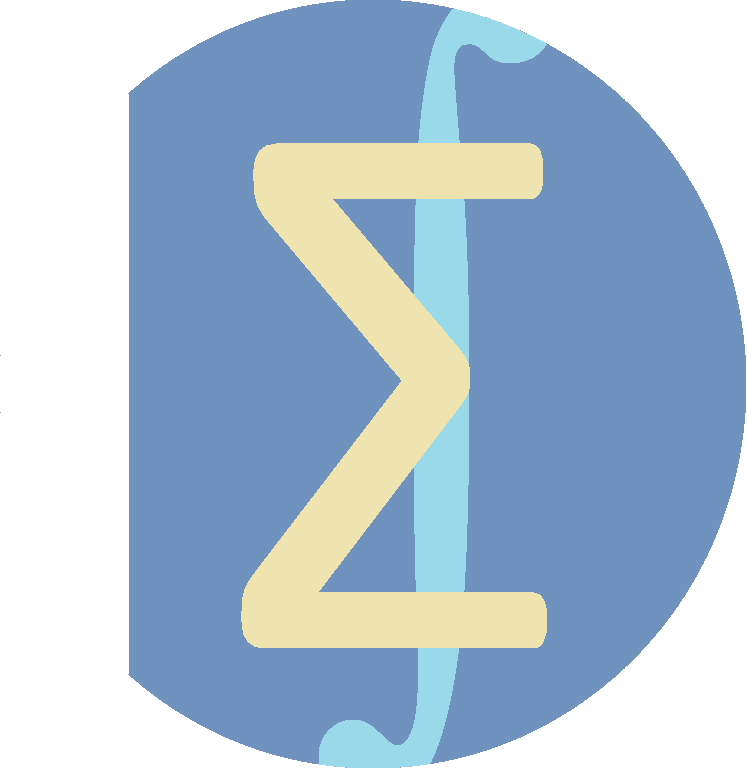
\includegraphics[width=1cm]{logo}
            
        \Large
        www.statmania.info\\
            
    \end{center}
\end{titlepage}

\tableofcontents

\newpage

\begin{questions}

\section{Basic Concept of Statistics}

\question \textbf{Who is known as the Father of modern statistics?}
\choice{P.C. Mahalanobis}{Kazi Motaher Hossain}{Karl Pearson}{R.A. Fisher}{d}

\question \textbf{Which is not a function of statistics?}
\choice{Data collection}{Data organization}{Analysis}{Database creation}{d}

\question \textbf{Which one is an example of an infinite population?}
\choice{Students of Dhaka University}{Cadets of SCC}
{Minor planets in the solar system}{Red blood cells in a person's body}{d}

\question \textbf{Which of the following is an example of an infinite population?}
\choice{Employees of a multinational company}{Trees in a national park}
{Stars in the Milky Way}{Passengers on a flight}{c}

\question \textbf{Which one represents an infinite population?}
\choice{Books in a library}{Fish in the Pacific Ocean}
{Members of a sports club}{Mobile phones in a city}{b}

\question \textbf{A researcher collected data on age and income of the 
people in a city. The variables are --}

i. bi-variate \\
ii. quantitative \\
iii. qualitative

\textbf{Which one is correct?}

\choice{i and ii}{i and iii}{ii and iii}{i, ii and iii}{a}

\question \textbf{Which of the following is correct?}
\choice{$\displaystyle \sum_{i=1}^{20} cx_i = nc \sum_{i=1}^{20} x_i$}
{$\displaystyle \sum_{i=1}^{20} cx_i = nc \sum_{i=1}^{20} x_i$}
{$\displaystyle \sum_{i=1}^{20} cx_i = c \sum_{i=1}^{20} x_i$}
{$\displaystyle \sum_{i=1}^{20} cx_i = c^2 \sum_{i=1}^{20} x_i$}{b}

\question \textbf{Which cannot be performed using Univariate data?}
\choice{Central tendency}{Dispersion}{Skewness}{Regression}{d}

\question \textbf{Which of the following cannot be analyzed using univariate data?}  
\choice{Mean}{Variance}{Correlation}{Range}{c}  

\question \textbf{Which statistical method requires bivariate or multivariate data?}  
\choice{Standard deviation}{Histogram}{Regression analysis}{Median}{c}  

\question \textbf{Which of the following is an example of an infinite population?}  
\choice{Patients in a hospital}{Water molecules in the ocean}  
{Cars on a highway}{Students in a university}{b}  

\question \textbf{Which one represents an infinite population?}  
\choice{Trees in a forest}{Grains of sand on a beach}  
{Books in a bookstore}{Houses in a neighborhood}{b}  


\question \textbf{Cities ranked according to habitability level show 
-- measurement scale}
\choice{Nominal}{Ratio}{Interval}{Ordinal}{d}

\question \textbf{Classifying students based on their grades (A, B, C, etc.) represents which measurement scale?}  
\choice{Nominal}{Ordinal}{Interval}{Ratio}{b}  

\question \textbf{Temperature measured in Celsius or Fahrenheit follows which type of measurement scale?}  
\choice{Nominal}{Ordinal}{Interval}{Ratio}{c}  

\question \textbf{A survey categorizing people by their favorite color is an example of which measurement scale?}  
\choice{Nominal}{Ordinal}{Interval}{Ratio}{a}  

\question \textbf{Which is not an example of shift of scale?}
\choice{$y_i = \frac{x_i}{a}$}{$y_i = cx_i$}{$y_i = x_i-2$}
{$y_i = \frac{cx_i}{d}$}{a}

\question \textbf{If $\displaystyle \sum_{i=1}^{20} x_i^2=20$ and
$\displaystyle \sum_{i=1}^{20} x_i=30$, what is the value of 
$\displaystyle \sum_{i=1}^{20} x_i^2 + \sum_{i=1}^{20} x_i + 100$?}
\choice{130}{200}{150}{2130}{c}

\question \textbf{If $\displaystyle \sum_{i=1}^{15} y_i^2=50$ and $\displaystyle \sum_{i=1}^{15} y_i=25$, what is the value of $\displaystyle \sum_{i=1}^{15} y_i^2 - \sum_{i=1}^{15} y_i + 75$?}  
\choice{100}{50}{125}{45}{a}  

\question \textbf{Given $\displaystyle \sum_{i=1}^{10} a_i^2=40$ and $\displaystyle \sum_{i=1}^{10} a_i=20$, find the value of $\displaystyle 2\sum_{i=1}^{10} a_i^2 - 3\sum_{i=1}^{10} a_i + 60$.}  
\choice{70}{100}{80}{50}{c}  

\question \textbf{If $\displaystyle \sum_{i=1}^{25} z_i^2=75$ and $\displaystyle \sum_{i=1}^{25} z_i=50$, compute $\displaystyle \sum_{i=1}^{25} z_i^2 + 2\sum_{i=1}^{25} z_i - 125$.}  
\choice{50}{75}{100}{25}{a}  


\question \textbf{A subset of a population is called--}
\choice{Constant}{Variable}{Sample}{Scale}{c}

\question \textbf{What is $\displaystyle \sum_{i=1}^n bx_i$ equal to?}
\choice{$\displaystyle b \sum_{i=1}^n nx_i$}
{$\displaystyle b \sum_{i=1}^n x_i$}
{$\displaystyle \sum_{i=1}^n nx_i$}{$\displaystyle bn \sum_{i=1}^n x_i$}{b}

\question \textbf{How many measurement scales are there?}
\choice{2}{3}{4}{5}{c}

\question \textbf{Which of the following is a continuous variable?}
\choice{Number of goals}{Natural number}{Summation of Fibonacci series}
{Success rate}{d}

\question \textbf{In which scale of measurement, zero is regarded as true zero?}
\choice{Nominal scale}{Interval scale}{Ratio scale}{Ordinal scale}{c}

\question \textbf{Which measurement scale does height belong to?}
\choice{Nominal}{Ordinal}{Interval}{Ratio}{d}

\question \textbf{Which is a discrete variable?}
\choice{Weight}{Amount of rainfall}{Distance}{Grade in a subject}{d}

\question \textbf{Which is a discrete variable?}
\choice{Height of a building}{Number of cars in a parking lot}
{Amount of milk in a container}{Time taken to complete a task}{b}

\question \textbf{Which is a discrete variable?}
\choice{Speed of a car}{Number of students in a class}
{Volume of water in a tank}{Temperature of a room}{b}

\question \textbf{Which is a discrete variable?}
\choice{Blood pressure}{Number of books on a shelf}
{Length of a river}{Amount of sugar in a cup}{b}

\question \textbf{Which is a discrete variable?}
\choice{Shoes sizes available in a store}{Distance between two cities}
{Volume of a gas}{Weight of a parcel}{a}

\question \textbf{Which is a discrete variable?}
\choice{Grades on a multiple-choice test (A, B, C, D)}
{Temperature during the day}{Height of a person}{Time spent on an activity}{a}

\question \textbf{Which is a discrete variable?}
\choice{Outcomes of rolling a die}{Speed of a train}
{Rainfall in a region}{Age of a tree}{a}

\question \textbf{Which is a discrete variable?}
\choice{Counts of people in a room}{Temperature recorded every hour}
{Weight of an animal}{Height of a plant}{a}

\question \textbf{Which is a discrete variable?}
\choice{Number of languages spoken by a person}
{Time taken to complete a race}{Length of a road}{Volume of water in a tank}{a}


\question \textbf{Which is a discrete variable?}
\choice{Length of a rope}{Weight of books in a library}{Distance}
{No. of particles in atoms}{d}

\question \textbf{$If x_1=2, x_2=-3, x_3=7$, and $x_4=12, 
\displaystyle \sum_{i=1}^4 x_i^2=?$}
\choice{26}{106}{206}{216}{c}

\question \textbf{If $x_1=5$, $x_2=-4$, $x_3=9$, and $x_4=0$, what is 
$\displaystyle \sum_{i=1}^4 x_i^2$?}  
\choice{82}{97}{107}{122}{d}  

\question \textbf{If $x_1=3$, $x_2=2$, $x_3=-6$, and $x_4=4$, what is
$\displaystyle \sum_{i=1}^4 x_i^2$?}  
\choice{45}{65}{85}{89}{b}

\question \textbf{If $x_1=4$, $x_2=1$, $x_3=-2$, and $x_4=3$, find 
$\displaystyle \sum_{i=1}^4 (x_i^2 + 3)$?}  
\choice{40}{50}{42}{56}{c}  

\question \textbf{If $y_1=5$, $y_2=2$, $y_3=-1$, and $y_4=4$, compute $\displaystyle \sum_{i=1}^4 (y_i^2 + 2)$.}  
\choice{50}{40}{44}{60}{c}  

\question \textbf{Given $z_1=3$, $z_2=0$, $z_3=-3$, and $z_4=2$, determine $\displaystyle \sum_{i=1}^4 (z_i^2 + 5)$.}  
\choice{30}{40}{35}{45}{d}  


\question \textbf{If $x_1=4$, $x_2=-2$, $x_3=1$, and $x_4=5$, calculate 
$\displaystyle \sum_{i=1}^4 (2x_i^2 - x_i)$?}  
\choice{38}{42}{46}{84}{d}  

\question \textbf{If $x_1=3$, $x_2=1$, $x_3=0$, and $x_4=2$, 
find $\displaystyle \sum_{i=1}^4 x_i^2 - \sum_{i=1}^4 x_i$?}  
\choice{7}{9}{8}{13}{c}  

\question \textbf{If $x_1=5$, $x_2=4$, $x_3=-3$, and $x_4=2$,
find $\displaystyle \sum_{i=1}^4 (x_i^2 + x_i)$?}  
\choice{58}{62}{66}{72}{b}  

\question \textbf{If $x_1=2$, $x_2=3$, $x_3=-1$, and $x_4=0$, 
calculate $\displaystyle \sum_{i=1}^4 (x_i^2 - 2)$?}  
\choice{0}{6}{8}{10}{b}  

\question \textbf{$If x_1=2, x_2=3, x_3=4, x_4=6$, and $x_5=5, 
\displaystyle \sum_{i=1}^4 x_i^2=?$}
\choice{80}{87}{90}{105}{c}

\question \textbf{If $f_i = 3, 5, 7$ and $x_i = 2, 4, 7$; ; 
what is the value of $\displaystyle \sum_{i=1}^3 f_ix_i^2$?}
\choice{450}{350}{345}{435}{d}

\question \textbf{If $f_i = 2, 4, 6$ and $x_i = 3, 5, 7$, what is the value of $\displaystyle \sum_{i=1}^3 f_ix_i^3$?}  
\choice{950}{1125}{2612}{1330}{c}  

\question \textbf{Given $f_i = 1, 3, 5$ and $x_i = 2, 4, 6$, find the value of $\displaystyle \sum_{i=1}^3 f_ix_i^4$.}  
\choice{1356}{1536}{1650}{7264}{d}  

\question \textbf{If $f_i = 3, 5, 7$ and $x_i = 2, 4, 6$, compute $\displaystyle \sum_{i=1}^3 f_ix_i^2$.}  
\choice{260}{280}{344}{320}{c}  


\question \textbf{Find the value of $\displaystyle \sum_{i=1}^{12} f_i(x_i-7)^2$ where $\displaystyle \sum_{i=1}^{12} f_ix_i^2=400, \sum_{i=1}^{12} f_ix_i=40, \sum_{i=1}^{12} f_i=10$}
\choice{320}{330}{250}{430}{b}

\question \textbf{If $x_1=3$, $x_2=-1$, $x_3=2$, and $x_4=0$, 
find $\displaystyle \sum_{i=1}^4 (x_i^3 + 2x_i)$?}  
\choice{12}{18}{24}{28}{c}  

\question \textbf{If $x_1=4$, $x_2=1$, $x_3=-2$, and $x_4=3$, 
calculate $\displaystyle \sum_{i=1}^4 (x_i^2 + 4x_i - 1)$?}  
\choice{16}{24}{34}{50}{d}  

\question \textbf{If $x_1=1$, $x_2=2$, $x_3=-3$, and $x_4=4$, 
find $\displaystyle \sum_{i=1}^4 (3x_i^3 - x_i^2)$?}  
\choice{108}{114}{-8}{201}{a}  

\question \textbf{If $x_1=5$, $x_2=0$, $x_3=-1$, and $x_4=2$, 
determine $\displaystyle \sum_{i=1}^4 (x_i^3 + x_i^2 + 3)$?}  
\choice{173}{174}{164}{172}{b}  


\question \textbf{Capital and profit belong to a variable which is--}

i. Bivariate \\
ii. Quantitative \\
iii. Qualitative

\textbf{Which one is correct?}

\choice{i and ii}{i and iii}{ii and iii}{i, ii and iii}{a}

\question \textbf{Which one falls in the category of interval scale?}
\choice {Temperature}{Speed}{Distance}{Film rating}{a}

\question \textbf{Which one falls in the category of nominal scale?}  
\choice{Height}{Temperature}{Gender}{Age}{c}  

\question \textbf{Which of the following is an example of an ordinal scale?}  
\choice{Temperature}{IQ Score}{Educational Level}{Weight}{c}  

\question \textbf{Which of the following is not example of a ratio scale?}  
\choice{Temperature}{Time}{Blood Pressure}{Speed}{a}  


\question \textbf{In which scale of measurement, zero is regarded as true zero?}
\choice{Nominal scale}{Interval scale}{Ratio scale}{Ordinal scale}{c}

\question \textbf{Which is a discrete variable?}
\choice{Weight}{Amount of rainfall}{Distance}{Grade in a subject}{d}

\question \textbf{Which one is product of square?}
\choice {$\prod x_i^2$}{$(\prod x_i)^2$}{$\sum x_i^2 \times \sum x$}{$\sum x_i^2$}{a}

\question \textbf{For which variable, determining number of terms is not possible?}
\choice{Discrete variable}{Continuous variable}{Quantitative variable}{Qualitative variable}{b}

\textbf{Answer the next three question based on the following information.}

\begin{center}
\textbf{A farmer collects growth (in cm) of 10 plants in a month and finds that \\ $\sum x_i = 7$ and $\sum x_i^2=15$}
\end{center}

\question \textbf{Which is considered statistics?}
\choice{Jaman obtained 75 in statistics}{Shafiq lives at Road no. 5}{Mean monthly income in a city is 60,000 taka}{Width of a book is 10 cm}{c}

\question \textbf{What is the value of $\sum (x_i+4)$ if x =\{2,3\}?}
\choice{23}{47}{22}{13}{d}

\question \textbf{If $\displaystyle x_1=2, x_2=3, x_3=5, x_4=7$ and $\displaystyle y_1=3, y_2=4, y_3=5, y_4=8; 
 \sum_{i=2}^4 x_iy_i=?$}
\choice{14}{201}{93}{117}{c}


\question \textbf{From the following table, $\displaystyle \sum_{i=1}^4 x_iy_i=?$}

\begin{table}[h]
\centering
\begin{tabular}{c|c|l|c|l}
X & 1  & 5  & 3 & 2  \\ \hline
Y & 20 & 12 & 3 & 14
\end{tabular}
\end{table}

\choice{14}{201}{99}{109}{c}

\question \textbf{What is the value of $\sum (x_i-4)^2$?}
\choice{23}{135}{484}{119}{d}

\question \textbf{If the square of summation is subtracted the sum of square, the value is - }
\choice{-8}{34}{8}{-34}{d}

\question \textbf{Which one is not an example of ratio scale?}
\choice{Room no.}{Income}{Number of accidents}{Weight}{a}

\question \textbf{Which one is discrete?}
\choice{Weight}{Amount of rainfall}{Temperature}{No. of member in a family}{d}

\question \textbf{Which type of scale of measurement are religion and blood group?}
\choice{Interval}{Ratio}{Nominal}{Ordinal}{c}

\textbf{Answer the next two questions based on the following information}

\begin{center}
$X = 20, 25, 30, 40$
\end{center}

\question \textbf{Find $\sum (X_i + 10)$}
\choice{150}{155}{125}{250}{b}

\question \textbf{$\displaystyle \sum (X_i-30)^2$}
\choice{225}{230}{420}{235}{a}

\textbf{Answer the next two questions based on the following information}

\begin{center}
$X = 3, 5, 7, 10$
\end{center}

\question \textbf{Find $\sum (X_i + 3)$}
\choice{28}{32}{37}{40}{c}

\question \textbf{$\displaystyle \sum (X_i-5)^2$}
\choice{16}{33}{12}{8}{b}

\textbf{Answer the next two questions based on the following information}

\begin{center} $X = 6, 8, 10, 12$ \end{center}

\question \textbf{Find $\sum (X_i - 4)$}
\choice{20}{30}{32}{22}{a}

\question \textbf{$\displaystyle \sum (X_i + 2)^2$}
\choice{196}{504}{210}{220}{b}

\textbf{Answer the next two questions based on the following information}

\begin{center} $X = 4, 9, 13, 15$ \end{center}

\question \textbf{Find $\sum (2X_i)$}
\choice{68}{70}{82}{74}{c}

\question \textbf{$\displaystyle \sum (X_i - 10)^2$}
\choice{71}{80}{85}{92}{a}

\textbf{Answer the next three questions based on the following information.}

The values of $x_i$ and $f_i$ are given below:

\begin{table}[h]
\centering
\begin{tabular}{c|c|c|c|c}
$x_i$ & 1     & 2     & 3     & 4     \\ \hline
$f_i$ & 2     & 3     & 4     & 1    
\end{tabular}
\end{table}

\question \textbf{Find $\displaystyle \sum_{i=1}^4 f_i x_i$.}  
\choice{20}{21}{22}{24}{d}  

\question \textbf{Compute $\displaystyle \sum_{i=1}^4 f_i x_i^2$.}  
\choice{30}{35}{66}{64}{c}  

\question \textbf{Determine $\displaystyle \sum_{i=1}^4 f_i^2 x_i$.}  
\choice{74}{49}{78}{65}{a}  

\textbf{Answer the next three questions based on the following information.}

The values of $x_i$ and $f_i$ are given below:

\begin{table}[h]
\centering
\begin{tabular}{c|c|c|c|c}
$x_i$ & 2     & 4     & 6     & 8     \\ \hline
$f_i$ & 2     & 2     & 5     & 4    
\end{tabular}
\end{table}

\question \textbf{Find $\displaystyle \sum_{i=1}^4 f_i x_i$.}  
\choice{50}{74}{56}{60}{b}  

\question \textbf{Compute $\displaystyle \sum_{i=1}^4 f_i x_i^2$.}  
\choice{256}{274}{476}{300}{c}  

\question \textbf{Determine $\displaystyle \sum_{i=1}^4 f_i (x_i-5)^2$.}  
\choice{61}{48}{52}{58}{a}  



%-----------------------------------Section 2

\section{Collection, Organization, and Presentation of Data}

%-----------------------------------Section 2

\question \textbf{How many sources of data are there?}
\choice{5}{4}{3}{2}{d}

\question \textbf{What is the raw material of research?}
\choice{Data}{Theory}{Graph}{Mean}{a}

\question \textbf{Data obtained through direct observation is called--}
\choice{Primary data}{Secondary data}{Original Data}{Informal data}{a}

\question \textbf{Which formula is used to find angles for Pie Chart?}
\choice{$\theta_i = \frac{f_i}{N}\times 100$}{$\theta_i = \frac{f_i}
{100}\times 360$}{$\theta_i = \frac{f_i}{N}\times 360$}
{$\theta_i = \frac{f_i}{N-1}\times 360$}{c}

\question \textbf{Who invented Stem and Leaf plot?}
\choice{Karl Pearson}{R.A. Fisher}{David Cox}{John Tukey}{d}

\question \textbf{If all the rats in Sylhet is a population, all the rats in Sylhet Airport is --}
\choice{Data}{Sample}{Statistics}{Frequency}{b}

\question \textbf{Which rule is suggested by H.G. Sturges for determining number of class (k)?}
\choice{$K=1+3.322logN$}{$K=1+3.222logN$}{$K=1-3.222logN$}{$K=1+2.332logN$}{a}

\question \textbf{To show runs per over in a cricket match, which diagram can be used?}
\choice{Histogram}{Bar Diagram}{Ogive}{Frequency polygon}{b}

%-------Situation Set Starts


%--------Group Starts
\textbf{Answer the next THREE questions based on the following information}

Radius of 80 trees are recorded and this frequency distribution is constructed.

\begin{table}[H]
\centering
\begin{tabular}{c|c|c|c|c}
\begin{tabular}[c]{@{}c@{}}Radius (cm)\end{tabular} & 0-10 & 10-20 & 20-30 & 30-40 \\ \hline
No. of Trees & 20 & 15 & 21 & 24
\end{tabular}
\end{table}

\question \textbf{How many trees have radius between 10 and 30?}
\choice{30}{15}{36}{21}{c}

\question \textbf{How many trees have radius at least 20?}
\choice{44}{45}{24}{21}{b}

\question \textbf{What percent of trees have radius between 20 and 40?}
\choice{44\%}{56\%}{46\%}{53\%}{a}
%----Group Ends

%--------Group Starts

\textbf{Answer the next THREE questions based on the following information.}

The heights of 100 plants were measured, and this frequency distribution was constructed.

\begin{table}[H]
\centering
\begin{tabular}{c|c|c|c|c}
\begin{tabular}[c]{@{}c@{}}Height (cm)\end{tabular} & 0-20 & 20-40 & 40-60 & 60-80 \\ \hline
No. of Plants & 25 & 30 & 20 & 25
\end{tabular}
\end{table}

\question \textbf{How many plants have height between 20 and 60?}
\choice{50}{30}{20}{25}{a}

\question \textbf{How many plants have height at least 40?}
\choice{50}{45}{40}{25}{b}

\question \textbf{What percent of plants have height between 20 and 80?}
\choice{80\%}{75\%}{60\%}{50\%}{b}
%----Group Ends

%--------Group Starts
\textbf{Answer the next THREE questions based on the following information.}

The weights of 120 fruits were recorded and this frequency distribution was constructed.

\begin{table}[H]
\centering
\begin{tabular}{c|c|c|c|c}
\begin{tabular}[c]{@{}c@{}}Weight (grams)\end{tabular} & 0-50 & 50-100 & 100-150 & 150-200 \\ \hline
No. of Fruits & 30 & 35 & 25 & 30
\end{tabular}
\end{table}

\question \textbf{How many fruits weigh at least 100 grams?}
\choice{55}{50}{60}{65}{a}

\question \textbf{How many fruits weigh less than 100 grams?}
\choice{68}{70}{65}{50}{c}

\question \textbf{What percent of fruits weigh between 50 and 150 grams?}
\choice{50\%}{55\%}{60\%}{75\%}{c}
%--------Group Ends

\textbf{Answer the next two questions based on the following information}

\begin{center}
\begin{table}[h]
\centering
\begin{tabular}{c|c|c|c|c}
Class Interval & <10     & 10-20     & 20-30     & 30-40     \\ \hline
Frequency & 6     & 3     & 7     & 4    
\end{tabular}
\end{table}
\end{center}

\question \textbf{What is relative frequency of the class with the highest
  frequency?}
\choice{0.25}{0.45}{0.40}{0.35}{d}

\question \textbf{Which curve is suitable for }
\choice{Histogram}{Bar Diagram}{Pie Chart}{Ogive}{d}
%--------Situation Set Ends

%---------Multiple Completion Starts

\question \textbf{Example of primary data ---}

i. A student collected data for research \\
ii. A professor had a studnet collect data for them \\
iii. A researcher collected data from a newspaper.

\textbf{Which one is correct?}

\choice{i and ii}{i and iii}{ii and iii}{i, ii and iii}{a}

\question \textbf{Which of the following is an example of secondary data?}

i. Data obtained from a published journal \\
ii. Data collected by a government agency and used by a researcher \\
iii. Data gathered directly through interviews

\textbf{Which one is correct?}

\choice{i and ii}{ii and iii}{i and iii}{i, ii and iii}{a}

\question \textbf{Which of the following represents primary data?}

i. A scientist collects soil samples for analysis \\
ii. Data compiled in a textbook \\
iii. A business owner surveys customers directly

\textbf{Which one is correct?}

\choice{i and iii}{i and ii}{ii and iii}{i, ii, and iii}{a}

\question \textbf{Which of these are examples of secondary data?}

i. A report sourced from census data \\
ii. A student conducting a direct experiment \\
iii. Statistics extracted from a government database

\textbf{Which one is correct?}

\choice{i and iii}{i and ii}{ii and iii}{i, ii, and iii}{a}

\question \textbf{Which one true of primary data?}

i. Original \\
ii. Suitable \\
iii. Reliable

\textbf{Which one is correct?}

\choice{i and ii}{i and iii}{ii and iii}{i, ii and iii}{d}

\question \textbf{Which statement is true about secondary data?}

i. Already published \\
ii. Economical \\
iii. Always up-to-date

\textbf{Which one is correct?}

\choice{i and ii}{i and iii}{ii and iii}{i, ii and iii}{a}

\question \textbf{Which one is true about secondary data?}

i. Easy to collect \\
ii. Collected by someone else \\
iii. Free from bias

\textbf{Which one is correct?}

\choice{i and ii}{i and iii}{ii and iii}{i, ii and iii}{a}

\question \textbf{Which is an advantage of primary data?}

i. Specific to the study \\
ii. More reliable \\
iii. Less time-consuming

\textbf{Which one is correct?}

\choice{i and ii}{i and iii}{ii and iii}{i, ii and iii}{a}

%---------Multiple Completion Ends

%-------------New Chapter
\section{Measures of Central Tendency}

%-----------------------------------------------------------------------
\subsection{General Questions}
%-----------------------------------------------------------------------

\question \textbf{Which statement is correct}
\choice{Quartiles are well defined}{Outliers affect Median}
{Median is always present in data}{Quadratic mean is widely used}{a}

\question \textbf{Which measure is suitable for open-ended distribution?}
\choice{Median}{Mode}{Geometric Mean}{Arithmetic mean}{b}

\question \textbf{Which is not a measure of central tendency?}
\choice{Arithmetic mean}{Mode}{Range}{Quadratic mean}{c}

\question \textbf{When is the statement $AM=GM=HM$ true?}
\choice{When the values are natural numbers}{When all the values are equal}{When all the values have equal frequency}{When mode is greater than median}{b}

\question \textbf{If a value is zero, which measure is not usable?}
\choice{Arithmetic Mean}{Harmonic Mean}{Geometrtic Mean}{Mode}{c}

\question \textbf{How many measure of central tendency are there?}
\choice{2}{3}{4}{5}{d}

\question \textbf{Which measure of central tendency is suitable for 
qualitative variable?}
\choice{Arithmetic Mean}{Harmonic Mean}{Quadratic Mean}{Mode}{d}

\question \textbf{In presence of negative values, which measure is not usable?}
\choice{Arithmetic Mean}{Geometric Mean}{Quadratic Mean}{Harmonic Mean}{b}

\textbf{Answer the next two questions based on the following information}


  \begin{table}[h]
\centering
\begin{tabular}{c|c|c|c|c|c}
Accident     & 4 & 6 & 7 & 8 & 9\\ \hline
Frequency & 2   & 0    & 4     & 5     & 1   
\end{tabular}
\end{table}
\question \textbf{Fifth Decile is --}
\choice{0}{8.5}{7.5}{8}{c}

\question \textbf{Which of the following is mode?}
\choice{4}{8}{0}{7}{b}

\question \textbf{Which measure always gives a value from within the values?}
\choice{Arithmetic Mean}{Geometric Mean}{Median}{Mode}{d}

\question \textbf{Which one is not a proper measure of central tendency?}
\choice{2nd Quartile}{Third Decile}{3rd Quintile}{110th Percentile}{d}

\question \textbf{Which one is smallest?}
\choice{$\displaystyle \sum_{i=1}^n (X_i-Median)^2$}{$\displaystyle 
\sum_{i=1}^n (X_i-\bar X)^2$}{$\displaystyle \sum_{i=1}^n (X_i-\sigma)^2$}
{$\displaystyle \sum_{i=1}^n (X_i-Mode)^2$}{a}

\question \textbf{Which measure is not used in determining skewness?}
\choice{Arithmetic Mean}{Geometric Mean}{Median}{Mode}{b}

\question \textbf{When is the relationship $AM = HM = GM$ true?}
\choice {All values are equal}{The values form a geometric progression}
{The values form an arithmetic progression}{All values are distinct}{a}

\question \textbf{In the presence of outlier(s), which measure of central 
tendency is suitable?}
\choice {Arithmetic mean}{Median}{Quadratic mean}{Power mean}{b}

\question \textbf{Which measure is suitable for dealing with population growth?}
\choice{Arithmetic Mean}{Geometric Mean}{Median}{Harmonic mean}{b}

\question \textbf{Which measure is best for calculating average rates of change over time?}  
\choice{Arithmetic Mean}{Geometric Mean}{Median}{Harmonic Mean}{b}  

\question \textbf{Which measure is best for determining average income in a highly skewed income distribution?}  
\choice{Arithmetic Mean}{Geometric Mean}{Median}{Harmonic Mean}{c}  

\question \textbf{Which can be measured from Ogive?}
\choice{Arithmetic Mean}{Geometric Mean}{Median}{Harmonic Mean}{c}  

\question \textbf{If a rate is defined as $\displaystyle R = \frac cd$, 
where c is constant, then which measure is perfect?}
\choice {Weighted arithmetic mean}{Harmonic mean}{Quadratic mean}
{Weighted geometric mean}{b}

\question \textbf{Which measure might have more than one value?}
\choice{Arithmetic mean}{Geometric mean}{Quadratic mean}{Mode}{d}

\question \textbf{Which relationship is correct?}
\choice{$AM \times GM = HM^2$}{$AM \times HM = GM^2$}{$AM \times HM = GM^3$}{$AM \div GM = HM^2$}{b}



\question \textbf{The arithmetic mean and geometric mean of two non-zero 
positive numbers are 15 and 10, respectively. What is harmonic mean?}
\choice{6.61}{6.67}{7.66}{6.76}{b}

\question 
\textbf{For two non-zero positive numbers, the harmonic mean is 8 and the geometric mean is 12. What is the arithmetic mean?}

\choice{16}{18}{20}{22}{b}

\question 
\textbf{For two non-zero positive numbers, the harmonic mean is 10 and the arithmetic mean is 25. What is the geometric mean?}

\choice{15}{20}{25}{30}{a}

%---------------------------------------------------------
\subsection{Arithmetic Mean}
%---------------------------------------------------------

\question \textbf{If $\sum (x_i-k)=0$, what is the value of k?}
\choice{$n$}{$\bar x$}{$x$}{$n \bar x$}{b}


\question \textbf{Find the arithmetic mean: $6, 9, 12, \cdots, 84$}
\choice{40}{45}{50}{55}{a}

\question \textbf{The arithmetic mean of first 10 natural numbers is:}
\choice{6}{8.5}{5.5}{5.6}{c}

\question \textbf{Arithmetic Mean of first 25 natural numbers is --}
\choice{12}{13}{14}{26}{b}

\question \textbf{An equation is: y = 5x + 9. If $\bar x = 20, \bar y = ?$}
\choice{100}{209}{109}{29}{c}

\question \textbf{Arithmetic Mean of two numbers is 25. If a number is 40, 
what is the other number?}
\choice{40}{50}{25}{10}{d}

\question \textbf{The Arithmetic Mean of two numbers is 30. If one number is 40, 
what is the other number?}
\choice{20}{30}{40}{60}{a}

\question \textbf{The Arithmetic Mean of two numbers is 35. If one number is 50, 
what is the other number?}
\choice{25}{20}{40}{70}{b}


\question \textbf{Number of students in two classes are 50 and 55 and their combined arithmetic mean (AM) of marks is 82. If AM of the first class is 75, what is the AM of the other class? }
\choice{88.36}{88.40}{84.55}{78.33}{a}

\question \textbf{The summation of deviation of each value from their 
arithmetic mean is --}
\choice{0}{1}{2}{4}{a}

\question \textbf{For grouped data, which formula is correct for Arithmetic Mean?}
\choice{$\displaystyle \bar X = \frac{\sum f_ix_i}{\sum f_i}$}{$\displaystyle \bar X = \frac{\sum x_i}{N}$}{$\displaystyle \bar X = \frac{\sum f_ix_i}{n}$}{$ \displaystyle\bar X = \frac{\sum f_i}{N}$}{a}

\question \textbf{Arithmetic mean of the series 2, 12, 22, $\cdots$, 92 is--}
\choice{45}{46}{47}{55}{c}

\question \textbf{What is the arithmetic mean of first n odd natural numbers?}
\choice{$\frac{n+1}{n}$}{n}{n+1}{$\frac{n+1}{2}$}{b}

\question \textbf{What is the arithmetic mean of first n even natural numbers?}
\choice{$\frac{n+1}{2}$}{$n+1$}{$n$}{$\frac{n-1}{2}$}{b}

\question \textbf{The arithmetic mean of first n natural numbers-}
\choice {$\frac{n}{2}$}{$\frac{n+1}{2}$}{$\frac{n^2}{2}$}{$\frac{n^2-1}{2}$}{b}

\question \textbf{Arithmetic means of three groups having equal no. of items are 30, 32, and 34. What is the combined mean?}
\choice{30.33}{32.67}{32.00}{33.00}{c}

%--------------------------------------------
\subsection{Harmonic Mean}

%--------------------------------------------

\question \textbf{Which formula is correct for harmonic mean?}
\choice{$\dfrac{n}{\sum_{i=1}^n \dfrac{f_i}{x_i}}$}{$\dfrac{f_i}{\sum_{i=1}^n \dfrac{f_i}{x_i}}$}{$\dfrac{\sum f_i}{\sum_{i=1}^n \dfrac{f_i}{x_i}}$}{$\dfrac{\sum f_i}{\sum_{i=1}^n \dfrac{1}{x_i}}$}{a}


\question \textbf{What is the harmonic mean of these values: 10, 12, 13, 15, 20, 25}
\choice{12.49}{14.93}{14.39}{13.49}{c}

\question \textbf{A rate is defined as $R = \frac c d;$  c and d are arbitrary numbers. If c is constant, which mean is used?}

\choice{Arithmetic Mean}{Geometric Mean}{Harmonic Mean}{Weighted Geometric Mean}{c}

\question \textbf{A rate is defined as $R = \frac c d;$  c and d are arbitrary numbers. If d is constant, which mean is used?}

\choice{Arithmetic Mean}{Geometric Mean}{Harmonic Mean}{Weighted Geometric Mean}{a}


\choice{Arithmetic Mean}{Geometric Mean}{Harmonic Mean}{Weighted Geometric Mean}{c}

\question \textbf{Which is the respresentation of Harmonic Mean?}
\choice{Mean of Reciprocal}{Reciprocal of Mean}{Reciprocal of Mean of Reciprocal}{None of the above}{c}

%--------------------------------------------
\subsection{Geometric Mean}
%--------------------------------------------

\question \textbf{Which data set is suitable for Geometric Mean?}
\choice{$1,-1,2,4,6,7$}{$1,2,4,8,16,32$}{$0,1,2,3,4,6$}{$1,1,2,3,4,4,5$}{b}

\question \textbf{Find geometric mean: 2, 4, 8, 16}
\choice{6.65}{6.56}{5.66}{5.56}{c}

\textbf{Answer the next three questions based on the following information}

\begin{center}
The data collected in a research is this: 1, 2, 4, 8, 16, 32
\end{center}

\question \textbf{Which measure is suitable?}
\choice{Arithmetic Mean}{Geometric Mean}{Median}{Mode}{b}

\question \textbf{What is the arithmetic mean of the data?}
\choice{8.5}{10}{8}{10.5}{d}

\question \textbf{What is the geometric mean?}
\choice{8.5}{5.66}{6.55}{16}{b}

\subsection{Mode}

\question \textbf{Which of the following may be used to determine mode?}
\choice{Histogram}{Frequency Curve}{Ogive}{Frequency Polygon}{a}

\question \textbf{What is the mode the set: 7, 8, 8, 9, 9, 13, 17, 9, 8, 8}
\choice{17}{9}{8}{Cqannot be determined}{c}

\subsection{Median}

\question \textbf{Which can be measured from the Ogive?}
\choice{Arithmetic Mean}{Geometric Mean}{Median}{Mode}{c}

\question \textbf{Median can be determined from the--}
\choice{Histogram}{Frequency curve}{Ogive}{Pie Chart}{c}

\subsection{Partition Values}

\subsection{Situation Set}

\textbf{Answer the next three questions based on the following information}

\textbf{The following table shows weekly production of milk (in liters) by different varieties of cows.}

\begin{center}
\begin{table}[h]
\centering
\begin{tabular}{c|c|c|c|c|c|c}
Interval     & 10-20 & 20-30 & 30-40 & 40-50 & 50-60 & 60-70 \\ \hline
Frequency    & 5     & 12    & 18    & 25    & 20    & 10    
\end{tabular}
\end{table} 
\end{center}

\question \textbf{What is the median?}
\choice{43}{44}{45}{50}{b}

\question \textbf{What is the lower limit of class interval for first quartile?}
\choice{10}{20}{30}{40}{c}

\question \textbf{What is the 3rd quartile?}
\choice{55.75}{43.75}{53.15}{53.75}{d}

\textbf{Answer the next two (2) questions based on the following information}

\begin{table}[h]
\centering
\begin{tabular}{c|c|c|c|c|c|c}
Class                                                           & $\le 20$ & 20-25 & 25-50 & 50-60 & 69-70 & $\ge 70$ \\ \hline
Frequency                                                       & 5        & 10    & 10    & 7     & 5     & 3        \\ \hline
\begin{tabular}[c]{@{}c@{}}Cumulative \\ Frequency\end{tabular} & 5        & 15    & 25    & 32    & 37    & 40      
\end{tabular}
\end{table}

\question \textbf{How many values are between 20 and 70?}
\choice{20}{32}{35}{37}{b}

\question \textbf{Which one is the median class?}
\choice{20-25}{25-50}{50-60}{60-70}{b}

\question \textbf{What is the median of the following values: 4, 5, 2, 1, 8, 3}
\choice{1.5}{2}{3.5}{4}{c}

\textbf{Answer the next three questions as per the following information.}

\begin{center}
42 44 59 64 70 72 74 91 94 are 9 values.
\end{center}

\question \textbf{What is the 50th percentile?}
\choice {64}{70}{72}{71}{b}

\question \textbf{Below which value lie 70 percent values?}
\choice {42}{44}{59}{74}{d}

\question \textbf{Above which value lie 30\% observations?}
\choice{3rd Quartile}{Median}{30th Percentile}{70th percentile}{d}

\textbf{Answer the next three questions as per the following information.}

\begin{center}
42 44 59 64 70 72 74 91 94 are 9 values.
\end{center}

\question \textbf{What is the median?}
\choice {64}{70}{72}{71}{b}

\question \textbf{What is the first quartile?}
\choice {42.4}{44.7}{51.5}{64.2}{c}

\question \textbf{Above which value lie 60\% observations?}
\choice{70.4}{72.0}{74.6}{66.4}{c}

\subsection{Multiple Completion}

\question \textbf{Inappropriate for algebraic analysis--}

i. Median \\
ii. Mode \\
iii. Geometric Mean

Which one is true?

\choice{i}{ii}{i \& ii}{ii \& iii}{c}

\question \textbf{With negative observations, which cannot be used}

i. Arithmetic Mean \\
ii. Geometric Mean \\
iii. Harmonic Mean

\textbf{Which one is correct?}

\choice{i and ii}{i and iii}{ii and iii}{i, ii and iii}{c}

\question \textbf{A good measure of central tendency -}

i. is loosly defined \\
ii. takes into consideration all values \\
iii. easily understandable

\textbf{Which one is correct?}

\choice{i and ii}{i and iii}{ii and iii}{i, ii and iii}{c}

\question \textbf{A good measure of central tendency -}  

i. is not affected by extreme values \\  
ii. represents the entire dataset accurately \\  
iii. is difficult to compute  

\textbf{Which one is correct?}  

\choice{i and ii}{i and iii}{ii and iii}{i, ii and iii}{a}  

\question \textbf{A good measure of central tendency -}  

i. is stable for different samples \\  
ii. provides a single representative value \\  
iii. ignores extreme values completely  

\textbf{Which one is correct?}  

\choice{i and ii}{i and iii}{ii and iii}{i, ii and iii}{a}  

\question \textbf{Median is --}  

i. Affected by extreme values \\  
ii. Rigidly defined \\  
iii. Suitable for open-ended distributions  

\textbf{Which one is correct?}  

\choice{i and ii}{i and iii}{ii and iii}{i, ii and iii}{b}  

\question \textbf{Mode is --}  

i. The most frequently occurring value \\  
ii. Unaffected by extreme values \\  
iii. Always unique in a dataset  

\textbf{Which one is correct?}  

\choice{i and ii}{i and iii}{ii and iii}{i, ii and iii}{a}  


\question \textbf{A rate is defined as $R = \frac c d;$  c and d are arbitrary numbers. If neither c or d is constant, which mean is used?}

i. Weighted Arithmetic Mean \\
ii. Weighted Harmonic Mean \\
iii. Harmonic Mean

\textbf{Which one is correct?}

\choice{i and ii}{i and iii}{ii and iii}{i, ii and iii}{a}

\question \textbf{What is true of harmonic mean?}

i. uses all values in tha data \\
ii. undefined if the any value is zero \\
iii. affected by extreme values

\textbf{Which one is correct?}

\choice{i and ii}{i and iii}{ii and iii}{i, ii and iii}{a}

\question \textbf{Arithmetic Mean is --}

i. Rigidly defined \\
ii. Unaffected by sample fluctuation \\
iii. Suitable for algebraic analysis

\textbf{Which one is correct?}

\choice{i and ii}{i and iii}{ii and iii}{i, ii and iii}{b}



\section{Measures of Dispersion}

\question \textbf{Which of the following is the best measure of dispersion?}
\choice{Range}{Mean deviation}{Standard deviation}{Coefficient of variation}{c}

\question \textbf{What is the minimum possible value of standard deviation?}
\choice{$\infty$}{-1}{0}{1}{c}

\question \textbf{For two values, range is found to be 8. What are the values of mean deviation and standard deviation}
\choice{(2,4)}{(4,4)}{(4,8)}{(8,8)}{a}

\question \textbf{What is the standard deviation of first 10 natural numbers?}
\choice{2.87}{3.02}{0}{2.78}{a}

\question \textbf{Which measure is unit-free?}
\choice{Range}{Mean deviation}{Standard deviation}{Coefficient of variation}{d}

\section{Moments, Skewness, and Kurtosis}

\subsection{Moments}

\question \textbf{Which is not a type of Moments}
\choice{Central Moments}{Raw Moments}{Corrected Moments}{Rectified Moments}{d}

\question \textbf{The second moment around w is --}
\choice{$\frac{\sum (x_i-\bar x)^n}{w}$}{$\frac{\sum (x_i-\bar x)^2}{w}$}{$\frac{\sum (x_i-w)^2}{n}$}{$\frac{\sum (x_i-w)^n}{2}$}{a}

\question \textbf{Which relatonship is correct?}
\choice{$\mu_1' = \bar x + a$}{$\mu_1' = \bar x - a$}{$\mu_2' = \bar x + a$}{$\mu_1 = \bar x - a$}{b}

\question \textbf{What is formula of rth raw moment for grouped data about a?}
\choice{$\frac{\sum f_i(x_i-a)^r}{n}$}{$\frac{\sum f_i(x_i-\bar x)^r}{n}$}{$\frac{\sum (x_i-a)^r}{n}$}{$\frac{\sum (x_i+a)^r}{n}$}{a}

\question \textbf{Which quantity uniquely characterizes a distribution?}
\choice{Median}{Quantile}{Moments}{Trend}{c}

\textbf{Which one is correct?}

\choice{i and ii}{i and iii}{ii and iii}{i, ii and iii}{d}

\question \textbf{Which can be used to measure dispersion?}
\choice{$\mu_2'$}{$\mu_1$}{$\mu_2$}{$\mu_1'$}{c}

\question \textbf{The formula of coefficient of variance (CV) is --}
\choice{$\frac{\sqrt{\mu_2}}{n}\times 100$}{$\frac{\mu_2}{\mu_1}\times 100$}{$\frac{\sqrt{\mu_2}}{\bar x}\times 100$}{$\frac{\mu_3}{\sigma}\times 100$}{c}

\question \textbf{First moment around zero is --}
\choice{0}{1}{-1}{Arithmetic Mean}{d}

\question \textbf{Which moment is equal to zero?}
\choice{First raw moment around 1}{Second central moment}{First central moment}{Second raw moment around 0}{c}

\question \textbf{Which might have a negative value?}
\choice{$\mu_4$}{$\mu_3$}{$\mu_2'$}{$\mu_2$}{b}

\question \textbf{2nd Central Moment is --}
\choice{$\mu_2-\mu_1'$}{$\mu_2+\mu_1'$}{$\mu_2-\mu_1'^2$}{$\mu_2'-\mu_1'^2$}{d}

\question \textbf{First central moment is equal to --}
\choice{1}{0}{-1}{$\bar x-a$}{b}

\question \textbf{First moment around a is equal to --}
\choice{1}{0}{-1}{$\bar x-a$}{d}

\question \textbf{The first raw moment about 3 is -5. What is the value of 
arithmetic mean?}
\choice{2}{-2}{0}{8}{b}

\question \textbf{The first raw moment about 4 is -4. What is the value of 
arithmetic mean?}
\choice{2}{-2}{0}{8}{c}

\question \textbf{The first raw moment about 0 is 2. What is the value of 
arithmetic mean?}
\choice{2}{-2}{0}{8}{a}

\question \textbf{The arithmetic mean of a variable is 4. What is the 
first raw moment around 2?}
\choice{2}{-2}{0}{8}{a}

\question \textbf{The arithmetic mean of a variable is 10. What is the 
first raw moment around 0?}
\choice{10}{-2}{0}{8}{a}

\question \textbf{The arithmetic mean of a variable is 2.6. What is the 
first raw moment around 6?}
\choice{2.2}{-3.4}{0.1}{1.8}{b}

\question \textbf{Moments can be--}

i. positive \\
ii. not negative \\
iii. positive or negative

\textbf{Which one is correct?}

\choice{i and ii}{i and iii}{ii and iii}{i, ii and iii}{b}

%------------------------------------------------------------------------------
\subsection{Skewness}
%------------------------------------------------------------------------------

\question \textbf{The following graph is an example of --}

\begin{center}
   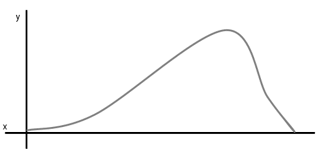
\includegraphics[width=0.2\textwidth]{../img/neg_skew.png}
\end{center}

\choice{Positive Skew}{Negative Skew}{No Skew}{Not detectable}{a}

%-------------------------------------STARTS Group

\textbf{Answer the next ? questions based on the following information}

\begin{center}
   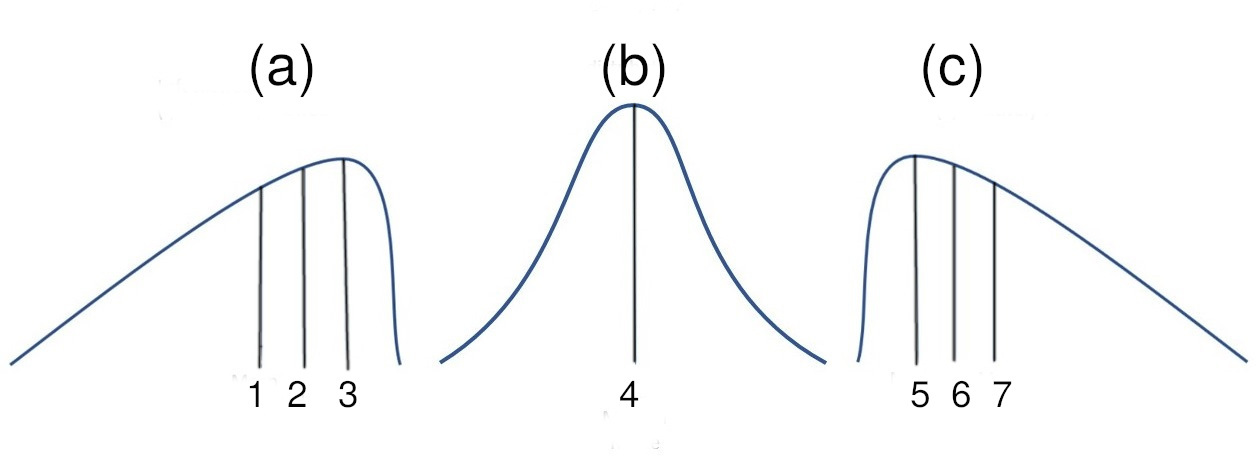
\includegraphics[width=0.5\textwidth]{../../slide/img/skewness_clean.jpg}
\end{center}

\question \textbf{The curve (a) is an example of}
\choice{Positive Skew}{Negative Skew}{No Skew}{Not detectable}{b}

\question \textbf{The curve (b) is an example of}
\choice{Positive Skew}{Negative Skew}{No Skew}{Not detectable}{a}

\question \textbf{In Image (b), what is denoted by 4th value?}
\choice{Mean}{Median}{Mode}{All of the above}{d}

\question \textbf{In Image (c), what is in 6th value?}
\choice{Mean}{Median}{Mode}{None of the above}{b}

\question \textbf{What is the value corresponding to the position 3?}
\choice{Mean}{Median}{Mode}{None of the above}{c}

\question \textbf{What is the value corresponding to the position 7?}
\choice{Mean}{Median}{Mode}{None of the above}{a}

%-------------------------------------ENDS Group

\question \textbf{If $\gamma_1 > 0$, the data is -}
\choice{Negatively skewed}{Positively skewed}{Symmetric}{Uncertain}{b}

\question \textbf{Which relationship is correct?}
\choice{$M_o = 2Me - \bar x$}{$M_o = 3Me - \bar x$}{$M_o = 3Me - 2 \bar x$}{$M_o = 2Me - 3 \bar x$}{c}

\question \textbf{Characteristics of a skewed distributon are --}

i. $Mean \ne Median \ne Mode$ \\
ii. Differences of upper and lower quartiles from median are unequal\\
iii. Frequency curve is asymmetric

\question \textbf{In a distribution, $\mu_2=25, \mu_3=20$, and $\mu_4=2200$; 
the distribution is --}
\choice{Negativelky skewed}{leptokurtic}{Platykurtic}{Symmetric}{b}

\question \textbf{For a data, $Q_3=41.6, Q_1=17.2, Median = 29, \& AM = 30$; What is Coefficient of skewness?}
\choice{24.4}{1}{0.03}{29.45}{d}

\question \textbf{In case of positive skewness, which one is correct?}
\choice{$Mean>Median>Mode$}{$Mean<Median<Mode$}{$Mean=Median=Mode$}
{$Mean>Median<Mode$}{a}

\question \textbf{For a symmetrical distribution, $\beta_1=$\textemdash}
\choice{1}{-1}{0}{3}{c}

\question \textbf{$\sqrt{\beta_1}=-0.23$ implies--}
\choice{Left Skew}{Symmetry}{Right Skew}{Mesokurtic}{a}

\question \textbf{$\gamma_1=0.43$ implies--}
\choice{Left Skew}{Symmetry}{Right Skew}{Mesokurtic}{c}

\question \textbf{$\gamma_1=0.0001$ implies--}
\choice{Left Skew}{Symmetry}{Right Skew}{Mesokurtic}{b}

\question \textbf{First 3 moments about 2 are 1, 2 and 8, respectively. 
What is the arithmetic mena?}
\choice{1}{2}{3}{4}{c}

\question \textbf{What is the second central moments of first 10 natural numbers?}
\choice{9.90}{9.09}{8.25}{5.67}{c}

\question \textbf{Frequencies of low and high values are smaller in -- distribution}
\choice{Positively skewed}{Negatively skewed}{Symmetric}{Mesokurtic}{c}

\question \textbf{Frequencies of higher values are smaller and of low values are
higher in -- distribution}
\choice{Positively skewed}{Negatively skewed}{Symmetric}{Mesokurtic}{a}

\question \textbf{Frequencies of higher values are higher and of low values are
lower in -- distribution}
\choice{Positively skewed}{Negatively skewed}{Symmetric}{Mesokurtic}{b}

\question \textbf{In a postively-skewed distribution--}

i. Frequencies of higher values are lower \\
ii. Frequencies of low values are higher \\
iii. Frequencies of higher values are higher

\textbf{Which one is correct?}

\choice{i and ii}{i and iii}{ii and iii}{i, ii and iii}{a}

\question \textbf{In a negatively-skewed distribution--}

i. Frequencies of higher values are lower \\
ii. Frequencies of low values are lower \\
iii. Frequencies of higher values are higher

\textbf{Which one is correct?}

\choice{i and ii}{i and iii}{ii and iii}{i, ii and iii}{c}

\question \textbf{In a symmetric distribution--}

i. Frequencies of higher values are lower \\
ii. Frequencies of low values are higher \\
iii. Frequencies of low values are lower 

\textbf{Which one is correct?}

\choice{i and ii}{i and iii}{ii and iii}{i, ii and iii}{b}

\question \textbf{Which formula is correct for determining skewness?}
\choice{$\gamma_1 = \sqrt{\frac{\mu_3^2}{\mu_2^3}}$}{$\gamma_1=\sqrt{\beta_1^2}$}{$\gamma_1 = \sqrt{\frac{\mu_3}{\mu_2^3}}$}{$\frac{\mu_2}{\sqrt{\mu_3^2}}$}{a}

\subsection{Kurtosis}

\question \textbf{Which curve is platykurtic?}

\begin{center}
   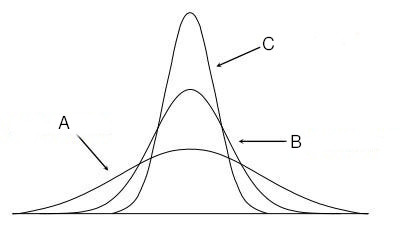
\includegraphics[width=0.4\textwidth]{../img/kurtosis.jpg}
\end{center}

\choice{A}{B}{C}{None}{a}

\question \textbf{How many types of kurtosis are there?}
\choice{2}{3}{4}{5}{b}

\question \textbf{The standard deviation of a mesokurtik distribution is 2. What is the value of the 4th central moment?}
\choice{4}{8}{16}{48}{d}

\question \textbf{$\beta_2 = \sqrt 9$ implies data are--}
\choice{Leptokurtic}{Platykurtic}{Mesokurtic}{Symmetric}{c}

\question \textbf{For a mesokurtik distribution, $\beta_2 = --$}
\choice{0}{-3}{3}{1}{c}

\question \textbf{What is the relationship between $\gamma_2$ and $\beta_2$?}
\choice{$\gamma_2 = \beta_2 + 3$}{$\gamma_2 = 2\beta_2 - 3$}{$\gamma_2 = \beta_2 - 1$}{$\gamma_2 = \beta_2 - 3$}{d}

\subsection{Misc}

\question \textbf{What is formula of the left inner fence for a box and whisker plot?}
\choice{$Q_1-1.5 \times IQR$}{$Q_3+1.5 \times IQR$}{$Q_1-3 \times IQR$}{$Q_3+1.5 \times IQR$}{a}

\question \textbf{What is the formula of IQR?}
\choice{$IQR = Q_3 + Q_1$}{$IQR = Q_3 - Q_1$}{$IQR = 2Q_3 - Q_1$}{$IQR = \frac{Q_3 - Q_1}{2}$}{b}

\question \textbf{Which is not used in constructing Box \& Whisker Plot?}
\choice{Mode}{$X_L$}{$Q_1 \& Q_3$}{$Q_1, Q_2 \& Q_3$}{a}

\question \textbf{In a symmatric distribution--}

i. Arithmetic Mean = Mode = Median \\
ii. $Q_2-Q_1 = Q_3-Q_2$  \\
iii. $Q_1-X_L = X_H-Q_3$

Which one is true?

\choice{i \& ii}{ii \& iii}{i \&iii}{i, ii \&iii}{d}

\question \textbf{Which is not included in five number summary?}
\choice{Arithmetic Mean}{$X_H$}{$Q_2$}{$Q_3$}{a}

\section{Correlation and Regression}


%------------------------------------------------------------------------------
\section{Time Series}
%------------------------------------------------------------------------------

\question \textbf{Which is not a time series data?}
\choice{Number of calls received per week}{No. of road accidents on 
different days}{No. of earthquakes in different regions}
{No. of particles decayed in each second}{c}

\question \textbf{Which is not a time series data?}
\choice{Daily closing prices of a stock}{Annual temperature records of a city}
{Number of students in a each class}
{Number of visitors to a website each day}{c}

\question \textbf{Which is an example of time series data?}
\choice{Number of calls received by a call center each month}
{Height of children at different ages}
{Tota salary of all employees at a company}
{Population of different countries in 2020}{a}


\question \textbf{Which is a type of trend?}

i. Linear trend \\
ii. Non-linear trend \\
iii. Cyclic trend

\textbf{Which one is correct?}

\choice{i and ii}{i and iii}{ii and iii}{i, ii and iii}{a}

\question \textbf{Which can measure trend most precisely?}
\choice{Graphical method}{Semi-average method}{Moving average method}
{Quarter-average method}{c}

\question \textbf{Which is the multiplicative time series model?}
\choice{$Y_t = T_t \times S_t \times C_t \times R_t$}
{$Y_t = T_t \times D_t \times C_t \times R_t$}
{$Y_t = T_t \times P_t \times C_t \times R_t$}
{$Y_t = T_t \times G_t \times C_t \times R_t$}{a}

\textbf{Answer the next two questions based on the following information}

Commodity wise export shipments (In million US\$) of Frozen and live 
fish in Bangladesh are given below. 


\begin{table}[h]
\centering
\begin{tabular}{c|c|c|c}
Months & 2022-23 (July-Dec) & 2023-24 (Jan-Jun) & 2022-23 (July-Dec) \\ \hline
Amount & 246.38 & 175.19 & 215.13
\end{tabular}
\caption{\label{usdrate}Source:\href{https://www.bb.org.bd/econdata/bop/exp_rcpt_merchandise.php}{BB} }
\end{table}

\question \textbf{Which component of time series is most evident?}
\choice{Irregular variation}{Cyclic variation}{Trend}{Seasonal variation}{d}

\question \textbf{Which value is most probable in the next period?}
\choice{200}{190}{130}{220}{b}

\question \textbf{A linear trend goes along a -- }
\choice{a curved line}{a wave}{straight line}{circle}{a}

\question \textbf{A non-linear trend goes along a --}
\choice{a curved line}{a wave}{a cubic pattern}{Any of the above}{d}

\question \textbf{Which measure of trend is subjective?}
\choice{Semi-average method}{Graphical method}{Moving average method}
{None of the above}{b}

\textbf{Answer the next THREE questions based on the following information}

\begin{table}[h]
\begin{tabular}{c|cccccccc}
Year & 2016 & 2017 & 2018 & 2019 & 2020 & 2021 & 2022 & 2023 \\ \hline
USD Exchange Rate & 78.35 & 79.49 & 82.87 & 83.26 & 84.60 & 84.37 & 85.80 & 106.70
\end{tabular}
\caption{\label{usdrate}Source--Investing.com}
\end{table}

\question \textbf{What is the second value of semi-average method?}
\choice{85.40}{90.37}{91.73}{89.78}{b}

\question \textbf{What kind of a trend do the data have?}
\choice{Upward}{Downward}{Both upward \& downward}{No trend}{a}

\question \textbf{Which component of time series is visible in the later 
part of the data?}
\choice{Seasonal Variation}{General Trend}{Irregular Variation}
{Cyclic Variation}{c}

% ----Group Starts

\textbf{Answer the next THREE questions based on the following information}

\begin{table}[h]
\begin{tabular}{c|cccccccc}
Year & 2016 & 2017 & 2018 & 2019 & 2020 & 2021 & 2022 & 2023 \\ \hline
USD Exchange Rate & 78.35 & 79.49 & 82.87 & 83.26 & 84.60 & 84.37 & 85.80 & 106.70
\end{tabular}
\caption{\label{usdrate}Source--Investing.com}
\end{table}

\question \textbf{What is the second value of semi-average method?}
\choice{85.40}{90.37}{91.73}{89.78}{b}

\question \textbf{What kind of a trend do the data have?}
\choice{Upward}{Downward}{Both upward \& downward}{No trend}{a}

\question \textbf{Which component of time series is visible in the 
later part of the data?}
\choice{Seasonal Variation}{General Trend}{Irregular Variation}
{Cyclic Variation}{c}

% ---- Group Ends

%-----------Group STARTS

\textbf{Answer the next THREE questions based on the following information}

\begin{table}[h]
\centering
\begin{tabular}{c|cccccccc}
Month & January & February & March & April & May & June & July & August \\ \hline
Rainfall (mm) & 150 & 120 & 180 & 200 & 160 & 140 & 170 & 190
\end{tabular}
\caption{\label{rainfalldata}Source: Meteorological Department}
\end{table}

\question \textbf{What is the semi-average for the second period of the data?}
\choice{160}{165}{180}{190}{b}

\question \textbf{Which type of trend do these rainfall data indicate?}
\choice{Increasing}{Decreasing}{No trend}{Fluctuating}{d}

\question \textbf{What is the primary variation component observed in the data?}
\choice{Seasonal Variation}{Trend Variation}{Cyclic Variation}
{Irregular Variation}{a}

% ---- Group Ends

\question \textbf{Time Series has how many components?}
\choice{2}{3}{4}{5}{c}

\question \textbf{Which component involves period more than one (01) year?}
\choice{Seasonal Variation}{Cyclic Variation}{Irregular Variation}{Random Variation}{b}

\question \textbf{Which one is not a component of Time Series}
\choice{Seasonal Variation}{Cyclic Variation}{General Trend}{Regular Variation}{d}

\question \textbf{A company is constantly getting greater revenue than previous year; this is--}
\choice{Seasonal Variation}{General Trend}{Irregular Variation}{Cyclic Variation}{b}

\question \textbf{Which is not a method of finding general trend?}
\choice{Graphical Method}{Moving Average}{Semi-Average}{Moving Median}{d}

% ---- Group Starts
\textbf{Answer the next two questions based on the following table:}

  \begin{table}[h]
\centering
\begin{tabular}{ccccccc}
Year     & 2007 & 2008 & 2009 & 2010 & 2011 & 2012\\ \hline
Sales & 5   & 35    & 34     & 40     & 42  & 204 
\end{tabular}
\end{table}

\question \textbf{In Semi-Average method, what is the 2nd average?}
\choice{74}{24.67}{95.33}{28}{c}

\question \textbf{What is the last  value of 3-yearly moving average?}
\choice{93.55}{95.53}{95.33}{59.33}{c}
% ---- Group Ends

\question \textbf{Which component of time series is affected by economic 
changes due to war?}
\choice{Trend}{Seasonal Variation}{Irregular Variation}{Cyclic Variation}{c}

\question \textbf{Which component of time series is affected by economic 
changes during a recession?}
\choice{Trend}{Seasonal Variation}{Irregular Variation}{Cyclic Variation}{c}

\question \textbf{Which component of time series is most likely to be 
impacted by weather conditions like a monsoon season?}
\choice{Trend}{Seasonal Variation}{Irregular Variation}{Cyclic Variation}{b}

\question \textbf{Which component of time series would be influenced by 
government policy changes such as tax reforms?}
\choice{Trend}{Seasonal Variation}{Irregular Variation}{Cyclic Variation}{d}


% ---- Group Starts

\textbf{Answer the next three questions based on the following table:}

\begin{table}[h]
\centering
\begin{tabular}{ccccccc}
Year     & 2016 & 2017 & 2018 & 2019 & 2020 \\ \hline
Car Sales & 1200 & 1500 & 1700 & 1600 & 1800   
\end{tabular}
\end{table}

\question \textbf{What is the first value of the 2-year moving average?}
\choice{1350}{1300}{1400}{1250}{a}

\question \textbf{What is the last value of the 3-year moving average?}
\choice{1600}{1670}{1630}{1750}{c}

\question \textbf{What is the semi-average for the first period of the data?}
\choice{1350}{1400}{1450}{1300}{a}

% ---- Group Ends

\question \textbf{Demand for warm clothes is higher in winter season ans
less in summer. Which component of time series deals with this change?}
\choice{Trend}{Seasonal Variation}{Irregular Variation}{Cyclic Variation}{b}

\question \textbf{Death rates of a country for 7 years are given below:}

\begin{table}[H]
\centering
\begin{tabular}{c|c|c|c|c|c|c|l}
Year & 2009 & 2010 & 2011 & 2012 & 2013 & 2014 & 2015 \\ \hline
Rate & 5    & 7    & 6    & 8    & 7    & 12   & 13  
\end{tabular}
\end{table}

\textbf{In semi-average method, which year will be excluded?}
\choice{2012}{2013}{ 2015}{2009}{b}

\question \textbf{Which component of time series represents a natural disaster?}
\choice{Seasonal Variation}{General Trend}{Irregular Variation}{Cyclic Variation}{c}

\question \textbf{How many models of time series are there to combine the components?}
\choice{2}{3}{4}{5}{a}

\question \textbf{Which one reflects an irregular variation?}
\choice{Fluctuation in production due to war}{Price hike due to famine}{Rise of Temperature to drought}{Any of the above}{d}

%-------------------------------------------------------------------------------
\section{Published Statistics in Bangladesh}
%-------------------------------------------------------------------------------


\question \textbf{Limitations of published statistics in Bangladesh are --}

i. Wrong data collection method \\
ii. Insufficient data \\
iii. Lack of proper training

\textbf{Which one is correct?}

\choice{i and ii}{i and iii}{ii and iii}{i, ii and iii}{d}

\question \textbf{How many sources of published statistics are there in Bangladesh?}
\choice{2}{3}{4}{6}{b}

\question \textbf{Bangladesh Bureau of Statistics collect -- }
\choice{Official statistics}{Non-official statistics}{Semi-official statistics}{None of the above}{a}

\question \textbf{Which statistics are published by an NGO?}
\choice{Official statistics}{Non-official statistics}
{Semi-official statistics}{None of the above}{c}

\question \textbf{The primary source of official statistics in Bangladesh is --}
\choice{WHO}{BBS}{CPD}{UNDP}{b}

\question \textbf{Which statistics are typically published by NGOs like World Wildlife Fund (WWF)?}
\choice{Official statistics}{Non-official statistics}{Semi-official statistics}{None of the above}{b}

\question \textbf{Which organization typically publishes non-official statistics in the field of health?}
\choice{UNICEF}{World Health Organization (WHO)}{World Bank}{United Nations (UN)}{a}

\question \textbf{In Bangladesh, a census is usually done every -- years}
\choice{20}{15}{10}{12}{c}

%\question \textbf{To complete the song, the last answer should be
%\choice{a}{b}{c}{d}{e} % Invalid answer choice

\end{questions}

\newpage  %Uncomment to put on new age
\bigskip

\begin{multicols}{4}
[
Answer Key: 
]
\showallanswers % Phil Hirschorn
\end{multicols}


\end{document}